\documentclass[conference]{IEEEtran}
\IEEEoverridecommandlockouts

\usepackage{cite}
\usepackage{amsmath,amssymb,amsfonts}
\usepackage{graphicx}
\usepackage{textcomp}
\usepackage{xcolor}
\usepackage{booktabs}
\usepackage{multirow}
\usepackage{float}
\usepackage{url}

\setlength{\textfloatsep}{8pt plus 2pt minus 2pt}
\setlength{\dbltextfloatsep}{8pt plus 2pt minus 2pt}
\setlength{\floatsep}{6pt plus 2pt minus 2pt}
\setlength{\intextsep}{6pt plus 2pt minus 2pt}
\setlength{\abovedisplayskip}{6pt plus 2pt minus 2pt}
\setlength{\belowdisplayskip}{6pt plus 2pt minus 2pt}
\setlength{\abovedisplayshortskip}{4pt plus 2pt minus 2pt}
\setlength{\belowdisplayshortskip}{4pt plus 2pt minus 2pt}

\def\BibTeX{{\rm B\kern-.05em{\sc i\kern-.025em b}\kern-.08em
    T\kern-.1667em\lower.7ex\hbox{E}\kern-.125emX}}

\begin{document}

\title{PDSSC: Progressive Digital Semantic Speech Communication at Extremely Low Bitrates With Speaker-Side Reference Guidance}

\author{
\IEEEauthorblockN{Hao Cheng}
\IEEEauthorblockA{
Beijing Jiaotong University \\
Beijing, China \\
24125150@bjtu.edu.cn
}
}

\maketitle

\begin{abstract}
Non-terrestrial networks (NTNs), together with their integration with terrestrial infrastructure, support speech services in remote, offshore, moving-platform, and emergency-response scenarios, where bandwidth is scarce, packet loss is prevalent, and real-time operation is required. In this regime, conventional speech codecs become inefficient at extremely low bitrates, while existing speech semantic communication methods still struggle to support extremely low-bitrate transmission, packet-loss robustness, and low-latency deployment within one framework. To address this problem, we propose Progressive Digital Semantic Speech Communication (PDSSC). PDSSC uses a layered discrete representation that transmits semantic content first and progressively supplements higher-layer detail, thereby supporting progressive transmission under extremely low bitrate constraints. It treats bitrate reduction and packet loss as a speaker-related restoration problem, addressed by a flow completion model leveraging same-speaker side information for effective low-cost recovery. A lightweight bitrate controller is also introduced for flexible deployment. Experimental results on LibriSpeech show that the proposed method achieves better perceptual quality than Opus while reducing transmission bitrate by 87.5\%, and exhibits stronger robustness under packet-loss conditions. A prototype implementation also demonstrates the feasibility of the proposed framework for real-time deployment.
\end{abstract}

\begin{IEEEkeywords}
digital semantic speech communication, extremely low-bitrate speech transmission, progressive transmission, packet-loss recovery, bitrate adaptation
\end{IEEEkeywords}

\section{Introduction}
Non-terrestrial networks (NTNs), together with their integration with terrestrial infrastructure, are increasingly envisioned as an important architecture for extending communication services beyond conventional ground coverage and toward more ubiquitous connectivity~\cite{3gpp_ntn,cheng2022sagin,ngmn_ntn}. In such systems, speech services are often needed in remote areas, maritime environments, moving platforms, and disaster-response scenarios, where communication typically relies on bandwidth-constrained packet-switched links with frequent packet loss and real-time requirements~\cite{guler2018semantic,xie2021deepsc}. Under these conditions, simultaneously maintaining speech intelligibility, naturalness, robustness, and low latency is difficult, especially when the available bitrate is extremely limited.

This difficulty is closely related to the mismatch between these link conditions and existing speech coding paradigms. Conventional speech codecs such as AAC and Opus~\cite{iso_aac,valin2012opus} are mature and practical, but they are primarily designed for faithful signal reconstruction and perceptual quality preservation. At extremely low bitrates, they still spend substantial rate on details that are less critical to intelligibility, and their performance further degrades under packet loss. Speech semantic communication offers a different direction by explicitly prioritizing understanding-relevant information rather than treating all signal details with similar transmission importance. However, existing methods still struggle to jointly support extremely low-bitrate transmission, packet-loss robustness, and low-latency operation in digital packetized systems.

Prior work has improved different parts of this problem. DeepSC-style methods and Deep Speech Semantic Transmission(DSST)~\cite{xie2021deepsc,xiao2023dsst} show the benefit of semantic-aware transmission, but their continuous representations are not naturally compatible with digital packetized links and usually require higher transmission and computation cost. Recent low-bitrate approaches move toward learned discrete representations, including neural speech codecs such as EnCodec~\cite{defossez2023encodec} and digital semantic communication schemes based on RVQ-style tokenization~\cite{chen2025rvqgan}. These methods improve digital compatibility and low-rate reconstruction quality, but their transmitted representations are not explicitly organized by transmission priority, which limits further bitrate reduction and the possibility of progressive transmission. Receiver-side generative restoration methods, including large-speech-model-based semantic communication~\cite{tian2025lsm} and packet-loss-oriented semantic communication such as Glaris~\cite{han2025esc}, improve recovery from incomplete reception. Their gains, however, often come with heavier inference cost, which makes low-latency deployment more difficult. Despite recent progress, achieving semantic intelligibility at extremely low bitrate together with efficient real-time deployment remains difficult. In addition, current systems offer limited support for progressive transmission.

These limitations motivate our approach. We propose Progressive Digital Semantic Speech Communication (PDSSC), a digital semantic speech communication framework for bandwidth-constrained packet-switched speech links. At the transmitter, PDSSC uses a layered discrete representation in which intelligibility-critical semantic information is sent first, while higher layers progressively supplement speaker-related and other residual acoustic detail. Under this design, the detail loss caused by active bitrate selection and the information loss caused by passive packet loss can be viewed as one speaker-related feature restoration problem, because both mainly appear as missing high-layer speaker-related detail at the receiver. In many target applications, the served user groups are relatively fixed, so the receiver can maintain a local speech library that provides same-speaker side information and enables a low-step flow completion model to recover this unified missing information more effectively and with lower inference cost. PDSSC also includes a lightweight automatic bitrate control module. Experiments show that the proposed framework performs well under extremely low-bitrate and packet-loss conditions while remaining practical to deploy.

The main contributions of this work are summarized as follows:
\begin{itemize}
\item A progressive digital semantic transmission framework for extremely low-bitrate speech communication, built on semantic-priority layered discrete representation to enable further bitrate reduction and progressive transmission within one digital framework.
\item A unified low-latency restoration framework that leverages same-speaker side information to recover speaker-related loss caused by both bitrate reduction and channel impairment.
\item A lightweight automatic bitrate controller that improves transmission flexibility and overall system efficiency, thereby supporting real-time deployment.
\item A shared residual block design reused across both the layered codec and the receiver-side flow completion network, which keeps the two-stage system compact and lets the frozen codec front end and the trainable completion model share a common local-feature parameterization.
\end{itemize}

Notation: Bold symbols denote vector- or tensor-valued quantities, calligraphic symbols denote sets or operators, and subscripts/superscripts indicate operating conditions or layer indices when needed.
\begin{itemize}
\item $x,\hat{x},x_{\mathrm{ref}}^{(j)}$: input speech waveform, reconstructed waveform, and receiver-side reference speech of speaker $j$.
\item $T,f_s,s,F,D,\rho$: waveform length, sampling rate, encoder downsampling factor, latent frame number, latent feature dimension, and latent frame rate, with $\rho=f_s/s$.
\item $E_{\phi}(\cdot),D_{\psi}(\cdot),\mathcal{Q}(\cdot),\mathcal{D}_{q}(\cdot)$: semantic encoder, semantic decoder, RVQ quantization operator, and RVQ dequantization operator.
\item $\mathbf{h},\widetilde{\mathbf{h}},\widehat{\mathbf{h}}$: complete latent, incomplete latent, and recovered latent representation.
\item $\mathbf{h}^{(l)},\mathbf{r}^{(l)},\mathbf{z}^{(l)},\mathbf{c}^{(l)}_{k}$: layer-$l$ input feature, RVQ residual, quantized codeword-index sequence, and RVQ codeword.
\item $\mathbf{Z},\mathbf{Z}_{N},\tilde{\mathbf{Z}}_{N,p}$: complete layered source description, transmitted source description, and received incomplete token observation.
\item $N,R(N),R,R_{\max},\mathcal{R}$: transmitted layer number, resulting source bitrate, bitrate operating point, available bitrate budget, and candidate bitrate set.
\item $p,\hat{p},\mathbf{M}^{(l)}_{N,p}$: packet loss rate, estimated packet loss rate, and frame-wise availability mask.
\item $f_{\theta}(\cdot),F_{\theta}(\cdot),\mathbf{e}_{\mathrm{spk}},\mathbf{h}_{\tau},\mathbf{v}^{\star}$: receiver-side latent recovery function, flow completion network, same-speaker side-information embedding, interpolated latent state, and target flow velocity.
\item $\mathbf{e}_{\mathrm{tch}},\mathbf{f}^{(1)}$: teacher semantic representation and projected first-layer latent feature for semantic distillation.
\item $\mathbb{R},\mathbb{E}[\cdot]$: real field and expectation operator.
\item $\odot,\|\cdot\|_1,\|\cdot\|_2$: element-wise multiplication/masking, $\ell_1$ norm, and $\ell_2$ norm.
\end{itemize}

The remainder of this paper is organized as follows. Section II presents the system model and problem formulation. Section III introduces the proposed method. Section IV describes the experimental setup. Section V reports the experimental results and analysis. Section VI concludes the paper.

\section{System Model and Problem Formulation}
This section establishes the end-to-end communication model and formulates active bitrate reduction and passive packet erasure as unified incomplete observation over the same layered latent hierarchy.
\begin{figure*}[!t]
\centering
\makebox[\textwidth][c]{
\includegraphics[width=0.98\textwidth]{paper_figs/fig1.png}}
\caption{Overall architecture of the proposed PDSSC system.}
\label{fig:system_model}
\end{figure*}
\noindent Fig.~\ref{fig:system_model} illustrates the overall communication setting. We consider a fixed user set $\mathcal{U}=\{1,\ldots,J\}$ communicating over a bandwidth-limited packet-erasure link, where the transmitter provides the active user identity and the receiver retrieves the corresponding reference speech $x_{\mathrm{ref}}^{(j)}$ from a local speech library as side information for paralinguistic-detail recovery. The end-to-end system therefore consists of a transmitter that generates and packetizes layered semantic tokens, a packet-erasure channel, and a receiver that reconstructs the latent representation and decodes the waveform with side-information-guided recovery. We now describe the transmitter-side layered source representation. The transmitter maps an input waveform $x$ to a latent sequence
\begin{equation}
\mathbf{h}=E_{\phi}(x),\qquad \mathbf{h}\in\mathbb{R}^{D\times F},
\end{equation}
with $F$ latent frames. The latent is discretized by an $L$-layer residual vector quantizer with codebook size $K$ into
\begin{equation}
\mathbf{Z}=\mathcal{Q}(\mathbf{h})=\left[\mathbf{z}^{(1)},\mathbf{z}^{(2)},\ldots,\mathbf{z}^{(L)}\right],
\end{equation}
The complete latent is reconstructed by summing the decoded contributions from all layers and then decoded by the shared semantic decoder $D_{\psi}(\cdot)$. At the system level, $\mathbf{Z}$ serves as the digital source description, while the semantic roles of different layers are introduced in Section III.
\par Bitrate adaptation is implemented by selecting how many leading RVQ layers are transmitted. With $N\in\{1,\ldots,L\}$ and $\mathbf{Z}_{N}=[\mathbf{z}^{(1)},\ldots,\mathbf{z}^{(N)}]$, the resulting source bitrate is
\begin{equation}
R(N)=N\rho\log_2 K .
\end{equation}
With $f_s=16$ kHz, $s=320$, and $K=1024$, we have $\rho=50$ frames/s, which gives $0.5N$ kbps, so the transmitted-layer number $N$ directly determines the operating bitrate. Before transmission, the selected tokens are semantically interleaved and packetized so that neighboring token positions are distributed across different packets, and the channel is modeled as a packet-erasure link with packet loss probability $p$. After packet loss, de-packetization, and de-interleaving, the receiver obtains an incomplete layered token observation $\tilde{\mathbf{Z}}_{N,p}$, whose dequantization yields
\begin{equation}
\widetilde{\mathbf{h}}=\mathcal{D}_{q}\!\left(\tilde{\mathbf{Z}}_{N,p}\right)
=\sum_{l=1}^{L}\mathbf{M}^{(l)}_{N,p}\odot \mathbf{h}^{(l)},\qquad
\widetilde{\mathbf{h}}\in\mathbb{R}^{D\times F},
\end{equation}
Unrevealed high-layer tokens and channel losses therefore lead to the same mathematical object, namely incomplete observation of the complete latent representation $\mathbf{h}$. In our layered representation, the missing part is dominated by higher-layer paralinguistic and residual acoustic information rather than the semantic backbone, which motivates a unified recovery framework in which the receiver reconstructs a complete latent representation from $\widetilde{\mathbf{h}}$:
\begin{equation}
\widehat{\mathbf{h}}=f_{\theta}(\widetilde{\mathbf{h}},x_{\mathrm{ref}}^{(j)},R),\qquad
\hat{x}=D_{\psi}(\widehat{\mathbf{h}}),
\end{equation}
The central problem is therefore to design a digital semantic source representation and a recovery function $f_{\theta}$ such that reduced-rate transmission and packet erasure can be handled within the same incomplete-observation framework.

\section{Proposed Method}
This section presents the proposed PDSSC framework from both architectural and training perspectives. The method consists of three coupled modules, namely a semantic-priority layered codec, a receiver-side low-step flow completion model, and a lightweight channel-adaptive bitrate controller, which are optimized in three successive stages. Stage I learns the layered codec, Stage II trains the completion model with the codec frozen, and Stage III fits the controller on RD samples generated by the frozen end-to-end pipeline.

\subsection{Semantic-Priority Layered Codec}
Standard RVQ performs residual coding over mixed speech features, but it does not guarantee that the lowest transmitted layers will preserve the semantic backbone first. As a result, under aggressive bitrate reduction, the retained representation may still lose information that is most critical to intelligibility. Our design therefore treats semantic disentanglement as the central objective of layered representation learning. Instead of relying on residual quantization alone to produce a useful ordering, we explicitly drive the first layer toward pretrained semantic features, so that the lowest layer captures content and context information as early as possible, while the higher layers are left to progressively encode speaker-related paralinguistic cues and other residual acoustic detail.

The key mechanism is first-layer semantic distillation. The encoder-decoder backbone adopts a SEANet-style architecture with a two-layer bidirectional LSTM at the encoder output and a two-layer unidirectional LSTM in the decoder. This combination preserves both local acoustic structure and longer-range temporal context before quantization. The residual block used in the encoder and decoder follows the standard two-layer residual design described earlier. Building on the notation in Section II, the encoder output has latent dimension $D=1024$. The dequantized feature of the first RVQ layer is linearly projected from the codec space to the 768-dimensional HuBERT teacher space, and a semantic distillation loss is imposed between the projected feature $\mathbf{f}^{(1)}\in\mathbb{R}^{768}$ and the teacher representation $\mathbf{e}_{\mathrm{tch}}\in\mathbb{R}^{768}$. We use
\begin{equation}
\mathcal{L}_{\mathrm{dist}}=-\log\sigma\!\left(\cos(\mathbf{f}^{(1)},\mathbf{e}_{\mathrm{tch}})\right)
\end{equation}
to pull the first RVQ layer toward the teacher semantic space. This constraint is the key to the semantic-priority hierarchy: it makes the lowest layer behave like a semantic backbone rather than a generic acoustic code. Once the semantic backbone is fixed early, the later RVQ layers naturally absorb what remains, including timbre-related, prosodic, and other semantically secondary detail. In this way, semantic distillation produces the desired semantic disentanglement, while residual quantization progressively distributes the remaining information across upper layers.

Under this design, RVQ serves as the mechanism that allocates residual information across layers. It is applied in the usual residual form~\cite{oord2017vqvae}:
\begin{equation}
\mathbf{r}^{(1)}=\mathbf{h},
\end{equation}
\begin{equation}
\mathbf{r}^{(l+1)}=\mathbf{r}^{(l)}-\mathbf{h}^{(l)}.
\end{equation}
\begin{equation}
\mathbf{h}^{(l)}=\mathbf{c}^{(l)}_{z^{(l)}},
\end{equation}
\begin{equation}
z^{(l)}=\arg\min_{k\in\{0,\ldots,K-1\}}\left\|\mathbf{r}^{(l)}-\mathbf{c}^{(l)}_k\right\|_2^2,
\end{equation}
In our implementation, we use $L=8$ RVQ layers and focus on the 1.0--4.0 kbps operating range.

In addition, $\mathcal{L}_{\mathrm{rec}}=\|x-\hat{x}\|_1$ constrains signal reconstruction quality, $\mathcal{L}_{\mathrm{mel}}$ preserves perceptually important spectral envelopes, $\mathcal{L}_{\mathrm{commit}}$ stabilizes RVQ code assignment, and $\mathcal{L}_{\mathrm{adv}}$ together with $\mathcal{L}_{\mathrm{fm}}$ improves local realism and harmonic detail through adversarial supervision. Stage I jointly trains the encoder, RVQ, and decoder end to end by minimizing
\begin{align}
\mathcal{L}_{\mathrm{codec}}&=\mathcal{L}_{\mathrm{adv}}+\mathcal{L}_{\mathrm{fm}}+
\lambda_{\mathrm{mel}}\mathcal{L}_{\mathrm{mel}}+\lambda_{\mathrm{rec}}\mathcal{L}_{\mathrm{rec}}\notag\\
&\quad+\lambda_{\mathrm{q}}\mathcal{L}_{\mathrm{commit}}+
\lambda_{\mathrm{dist}}\mathcal{L}_{\mathrm{dist}}.
\end{align}
This objective induces the desired layerwise separation behavior: the first layer preferentially captures intelligibility-critical content and context information, whereas the subsequent RVQ layers encode the remaining reconstruction factors, including speaker-dependent paralinguistic cues, prosodic variation, fine spectral detail, and other utterance-specific residual attributes. Unlike two-branch designs that enforce factor separation through architectural duplication, our method achieves semantic disentanglement and transmission-priority-oriented separation inside a single layered codec. After Stage I, the trained encoder-decoder is frozen and used as the shared front end for both transmission and receiver-side completion. Fig.~\ref{fig:codec_arch} summarizes the codec architecture, residual block structure, and Stage-I training path.

\begin{figure}[!t]
\centering
\makebox[\linewidth][c]{
\includegraphics[width=1.00\linewidth]{paper_figs/fig2.png}}
\caption{Architecture of the semantic-priority layered codec.}
\label{fig:codec_arch}
\end{figure}

\subsection{Low-Step Flow Completion With Speaker-Side Information}
Direct decoding of the received partial layered description cannot recover complete speech information when higher layers are not transmitted or when packet erasures occur. Since bitrate-induced layer omission and channel loss can both be viewed as incomplete observation over the same latent hierarchy, we introduce a low-step flow completion model at the receiver to restore the missing residual detail while keeping inference short enough for real-time operation. For the active speaker $j$, the receiver retrieves the reference utterance $x_{\mathrm{ref}}^{(j)}$ from the local speech library and encodes it with a pretrained speaker encoder to obtain $\mathbf{e}_{\mathrm{spk}}$. In our implementation, a frozen GE2E-style backbone first extracts a speaker representation, followed by a trainable projection and normalization layer. This embedding is combined with a 128-dimensional sinusoidal time embedding and the bitrate condition $R$ to form a unified conditioning signal that modulates the residual blocks of the flow network, whose residual-block structure is the same as that used in the layered codec. The reference speech does not provide lexical content; instead, it steers completion toward speaker-consistent paralinguistic and fine acoustic details.

During Stage II, the frozen codec and channel simulator generate incomplete-complete latent pairs $(\widetilde{\mathbf{h}},\mathbf{h})$ under jointly sampled bitrate and packet-loss conditions. A random continuous time variable $\tau\sim\mathcal{U}(0,1)$ is sampled, and
\begin{equation}
\mathbf{h}_{\tau}=(1-\tau)\widetilde{\mathbf{h}}+\tau\mathbf{h},
\qquad
\mathbf{v}^{\star}=\mathbf{h}-\widetilde{\mathbf{h}}.
\end{equation}
Sampling $\tau$ over $[0,1]$ lets the network learn the corresponding time-conditioned velocity field over the full trajectory. The target velocity follows directly from the straight-line interpolation path, since $d\mathbf{h}_{\tau}/d\tau=\mathbf{h}-\widetilde{\mathbf{h}}=\mathbf{v}^{\star}$. Under the layered masking model, it can also be written as
\begin{equation}
\mathbf{v}^{\star}=
\sum_{l=1}^{L}\left(1-\mathbf{M}^{(l)}_{N,p}\right)\odot \mathbf{h}^{(l)},
\end{equation}
which shows that the learned velocity corresponds to the missing latent residual components caused by layer truncation and packet erasure. The completion model is therefore trained to restore missing layered residual information on top of the preserved semantic backbone, rather than to regenerate the entire speech representation from scratch. The model predicts the conditional vector field
\begin{equation}
\mathbf{v}_{\theta}=F_{\theta}(\mathbf{h}_{\tau},\tau,\mathbf{e}_{\mathrm{spk}},R),
\end{equation}
The training objective is
\begin{equation}
\mathcal{L}_{\mathrm{flow\text{-}comp}}=\mathbb{E}\!\left[w(R)\left\|\mathbf{v}_{\theta}-\mathbf{v}^{\star}\right\|_2^2\right]+\lambda_{\mathrm{stft}}\mathcal{L}_{\mathrm{mrstft}},
\end{equation}
which trains the network in flow-matching form~\cite{lipman2023flow} to predict the missing latent residual. The side information $\mathbf{e}_{\mathrm{spk}}$ and bitrate condition $R$ do not change the target velocity, but improve its conditional prediction across speakers and bitrate operating points. To emphasize harder low-rate cases, we set $w(R)=\max\!\left(1,\frac{5-R}{2}\right)+\delta\,\mathbf{1}[R=1.0\ \mathrm{kbps}]$, with an extra boost on the 1 kbps operating point. In Stage II, the codec is frozen, $R$ is sampled from 1.0 to 4.0 kbps with explicit bias toward the lowest-rate regime, and the packet loss probability is sampled from 0 to 30\%. In our implementation, the semantic-first operating point is kept reliable during flow-completion training, whereas packet loss is injected into the supplementary residual information. Multi-resolution STFT regularization is further used to constrain local spectral continuity and missing fine acoustic detail.

At inference time, a low-step Euler solver completes the latent representation:
\begin{equation}
\widehat{\mathbf{h}}^{(k+1)}=\widehat{\mathbf{h}}^{(k)}+\Delta \tau\,F_{\theta}(\widehat{\mathbf{h}}^{(k)},\tau_k,\mathbf{e}_{\mathrm{spk}},R),
\end{equation}
initialized from $\widehat{\mathbf{h}}^{(0)}=\widetilde{\mathbf{h}}$. Because the flow starts from an already informative incomplete latent rather than pure noise, the completion path is substantially shorter than unconditional generation, which makes low-step inference sufficient for this task. Fig.~\ref{fig:timbreflow_arch} shows the internal structure of the completion module and the corresponding Stage-II training path. 

\begin{figure}[!t]
\centerline{
\includegraphics[width=0.88\linewidth]{paper_figs/fig3.png}}
\caption{Architecture and Stage-II training of the low-step flow completion module.}
\label{fig:timbreflow_arch}
\end{figure}

Both stages of PDSSC are assembled from a common residual block, whose internal structure is shown in Fig.~\ref{fig:resblock}. The block follows a two-convolution residual topology: a residual branch applies two stacked 1-D convolutions and projects back to the input channel dimension, and its output is added to a skip connection that preserves the input. In Stage~I, this unit is instantiated as a SEANet-style residual block: an ELU activation precedes each convolution (with kernels of size 3 and 1), the intermediate width is compressed to half the channel dimension to reduce cost, the convolutions are weight-normalized, and a true identity skip is used. In Stage~II, the same residual topology is reused inside the flow completion network with two dilated 3-kernel convolutions; to inject the conditioning signal, a feature-wise linear modulation (FiLM) layer applies a speaker-, time-, and bitrate-dependent affine transform to the intermediate features, while GroupNorm together with SiLU replaces weight normalization and ELU so that the block stays stable under conditional generation. Reusing one residual design across both stages keeps the parameterization compact and lets the frozen codec front end and the trainable completion network share a common local-feature vocabulary.

\begin{figure}[!t]
\centerline{\includegraphics[width=0.85\linewidth]{paper_figs/fig10.png}}
\caption{Internal structure of the shared residual block used in both the layered codec (Stage~I) and the flow completion network (Stage~II).}
\label{fig:resblock}
\end{figure}

\subsection{Channel-Adaptive Bitrate Control}
To avoid the complexity of manual bitrate switching and improve transmission efficiency, we design a lightweight channel-adaptive bitrate controller. Because the transmitted bitrate is determined by how many leading RVQ layers are selected, channel adaptation can be formulated directly over bitrate operating points. Given the estimated packet loss rate $\hat{p}$ and the available source-rate budget $R_{\max}$, the controller minimizes
\begin{equation}
\mathcal{J}(R,\hat{p})=\hat{D}_{\omega}(R,\hat{p})+\lambda_R R,
\label{eq:rd_cost}
\end{equation}
where the predicted distortion after channel degradation and receiver-side completion is given by $\hat{D}_{\omega}(R,\hat{p})$. The bitrate decision is then
\begin{equation}
R^{\star}(\hat{p})=\arg\min_{R\in\mathcal{R}} \mathcal{J}(R,\hat{p})
\quad \text{s.t.}\quad R\le R_{\max},
\label{eq:rd_rule}
\end{equation}
over $\mathcal{R}=\{0.5,1.0,\ldots,4.0\}$ kbps.

To train the controller, we freeze the codec and the completion model, sample utterances and packet loss rates, and evaluate the trained end-to-end pipeline over all candidate bitrate operating points. For each utterance $x$ and channel condition $p$, this produces a set of realized distortions
\begin{equation}
D^{\star}(x,R,p)=d\!\left(\hat{x}(x,R,p),x\right).
\end{equation}
The controller is parameterized by a small policy network that takes $\hat{p}$ together with $R_{\max}$ as input and outputs a score over candidate bitrate operating points. During training, the score vector is converted to a soft decision distribution
\begin{equation}
\pi_{\omega}(R|\hat{p},R_{\max})=\frac{\exp(-\hat{D}_{\omega}(R,\hat{p})/T_c)}{\sum_{r\in\mathcal{R}}\exp(-\hat{D}_{\omega}(r,\hat{p})/T_c)},
\end{equation}
We then optimize the expected RD objective
\begin{equation}
\begin{aligned}
\mathcal{L}_{\mathrm{ctrl}}
=\mathbb{E}_{x,p}\!\Big[
\sum_{R\in\mathcal{R}}\pi_{\omega}(R|p,R_{\max})
\left(D^{\star}(x,R,p)+\lambda_R R\right)
\Big].
\end{aligned}
\label{eq:ctrl_loss}
\end{equation}
In Stage III, the codec and completion model are frozen, and the controller is trained with \eqref{eq:ctrl_loss} on RD samples from the end-to-end system; deployment then uses the hard bitrate decision in \eqref{eq:rd_rule}.

\section{Experimental Setup}
This section describes the experimental settings used to evaluate PDSSC. All experiments are conducted on LibriSpeech, with the layered codec and the receiver-side flow completion model trained on \texttt{train-clean-100} and the main results reported on \texttt{test-clean}~\cite{panayotov2015librispeech}. Model training is performed on four NVIDIA A40 GPUs, whereas evaluation and latency measurement are conducted on a single NVIDIA RTX 3090 workstation. The overall training time is about 50 hours.

The proposed method is evaluated from 1.0 to 4.0 kbps at 0.5 kbps intervals. Unless otherwise stated, packet loss is implemented as Bernoulli random erasure on transmitted token frames. Comparisons are conducted against conventional speech codecs AAC and Opus, the neural codec EnCodec, and the recent low-bitrate semantic baseline ESC. To ensure fair comparison under packet-loss channels, Opus is evaluated with LBRR, while AAC, EnCodec, and ESC are equipped with LFR-PLC. ViSQOL~\cite{hines2015visqol} and UTMOS~\cite{saeki2022utmos} are used in the quality-bitrate experiments to assess objective speech quality and perceptual naturalness, respectively, whereas packet-loss robustness is evaluated by ViSQOL together with PLCMOS~\cite{diener2023plcmos}, a non-intrusive perceptual metric designed for packet-loss concealment. In the robustness experiments, PDSSC is tested at average 1.5 and 3.0 kbps, while the competing methods are evaluated at their corresponding operating points, including higher-rate protected baselines such as Opus at 8.0 kbps.

\section{Experimental Results and Analysis}
This section reports the experimental results and analyzes the behavior of PDSSC from several complementary perspectives. We examine the quality-bitrate tradeoff, robustness under packet loss, qualitative time-frequency reconstruction behavior, and practical deployment efficiency, and we further use feature visualization and ablation results to interpret the source of the observed gains.
We first analyze the quality-bitrate tradeoff under a fixed packet loss rate of 5\%, as shown in Fig.~\ref{fig:rate}. ViSQOL and UTMOS measure objective speech quality and perceptual naturalness, respectively. PDSSC is particularly advantageous in the extremely low-bitrate regime, where the source representation must decide what should be transmitted first and what can be deferred. As shown in the insets, PDSSC already surpasses ESC at several neighboring operating points while using fewer bits. For example, at 1.0 kbps, PDSSC reaches 3.859 in ViSQOL and 2.914 in UTMOS, already exceeding ESC at 1.5 kbps, which attains 3.834 and 2.861, respectively. A similar margin remains at higher neighboring points: PDSSC reaches 4.206 in ViSQOL at 2.5 kbps, above ESC at 3.0 kbps (4.151), while its UTMOS at 2.5 kbps is 3.721, clearly higher than the 3.280 achieved by ESC at 3.0 kbps. This comparison matters because ESC is not a weak reference, but one of the strongest existing semantic speech codecs in the 1.5 kbps and nearby low-rate region, and it is already equipped with packet-loss protection. PDSSC still improving over such a protected low-rate baseline indicates a genuine gain in representation efficiency rather than a superficial coding advantage.

The broader comparison with the remaining baselines leads to the same conclusion. Compared with conventional speech codecs, PDSSC reaches similar or better quality at much lower bitrate, indicating more effective use of the limited transmission budget. Relative to EnCodec, the advantage is more revealing: both systems are discrete neural codecs, but PDSSC maintains a markedly better quality-bitrate tradeoff in the low-rate region. The gain therefore does not come merely from replacing a conventional codec with a neural one, but from reorganizing the transmitted information into a progressively structured semantic hierarchy and then compensating the omitted residual detail at the receiver.

\begin{figure}[!t]
\makebox[\linewidth][c]{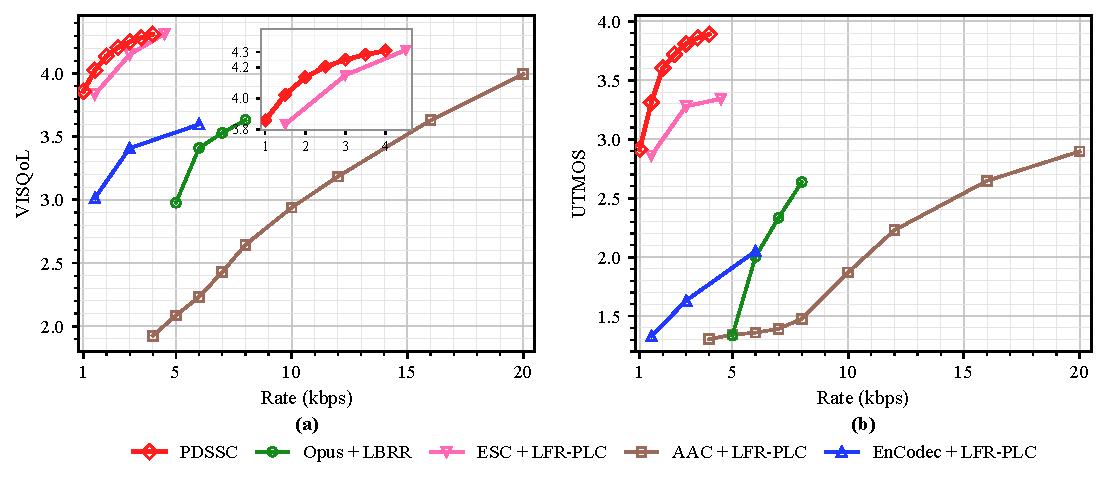
\includegraphics[width=1.05\linewidth]{paper_figs/fig4.pdf}}
\caption{Audio quality performance of PDSSC and competing methods at different bitrates under 5\% packet loss: (a) ViSQOL, (b) UTMOS.}
\label{fig:rate}
\end{figure}

Feature visualization helps explain why this quality-bitrate advantage emerges. Fig.~\ref{fig:disentangle} provides a feature-space visualization across quantization layers. For PDSSC, the first layer is widely and relatively uniformly distributed across speakers, which suggests that it has largely discarded speaker-dependent variation and retained a more speaker-invariant semantic organization. The later-layer aggregation shows the opposite tendency: speaker-related structure becomes much more concentrated there, indicating that the higher layers progressively absorb paralinguistic and other semantically irrelevant residual attributes. By contrast, the EnCodec features remain more strongly coupled across layers. Its early-layer representation does not isolate semantic content as clearly, while the higher-layer aggregation still carries information that is not fully decoupled from the lower-layer structure. This weaker disentanglement means that bitrate reduction in EnCodec removes semantic and non-semantic information together, rather than predominantly trimming semantically irrelevant detail. PDSSC instead enforces a clearer progressive separation between semantic and non-semantic factors, so reducing the transmitted bitrate mainly suppresses refinable residual content while preserving the part most critical to intelligibility. The visualization therefore offers a structural explanation for the superiority observed in Fig.~\ref{fig:rate}.


\begin{figure}[!t]
\makebox[\linewidth][c]{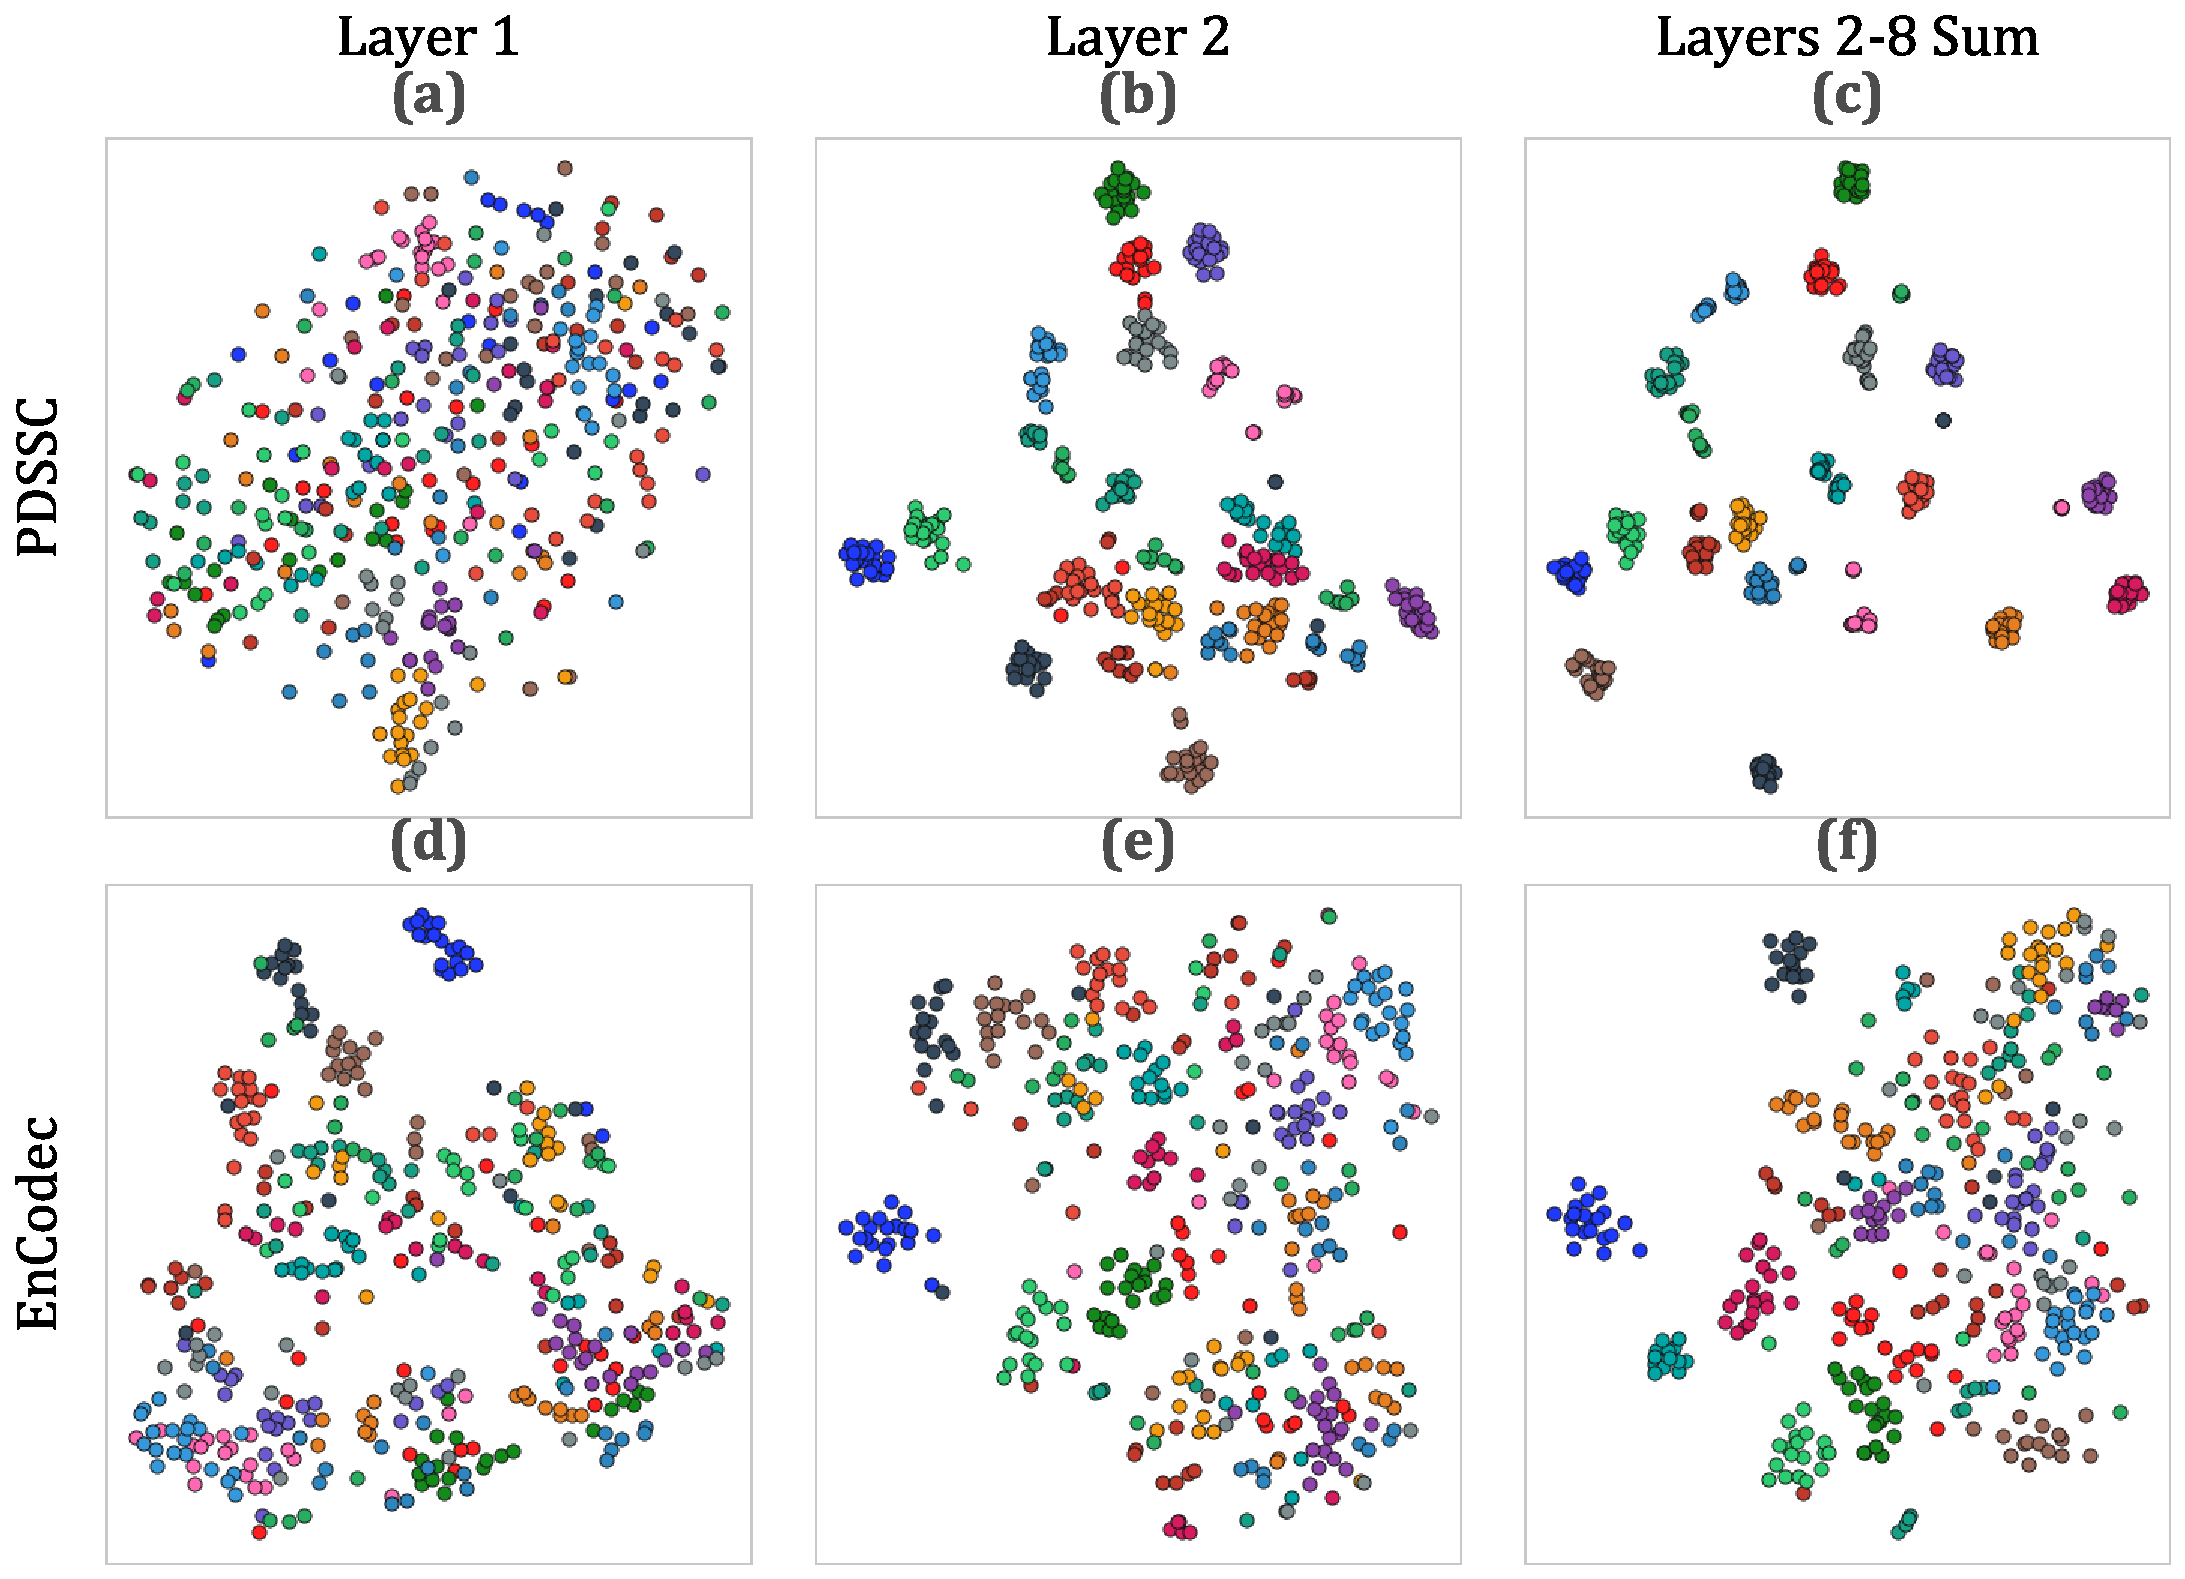
\includegraphics[width=1.05\linewidth]{paper_figs/fig5.pdf}}
\caption{Layer-wise feature visualization of PDSSC and EnCodec: first layer, second layer, and summed Layers 2--8.}
\label{fig:disentangle}
\end{figure}

We next examine robustness under increasing packet loss, as shown in Fig.~\ref{fig:plr}. Here, ViSQOL again measures overall speech quality, while PLCMOS is included because it is a non-intrusive perceptual metric specifically designed for packet-loss concealment conditions. PDSSC degrades much more gracefully than the competing methods as the channel becomes unreliable. Under both bitrate reduction and packet erasure, the missing components are dominated by higher-layer speaker-related and other semantically irrelevant residual attributes, while most of the semantic backbone is still preserved in the received latent representation. The receiver-side flow completion model is therefore highly targeted: rather than regenerating speech from scratch, it uses same-speaker prior knowledge to compensate for the missing high-layer detail on top of an already informative latent observation. Because the completion objective is always to recover the original full latent $\mathbf{h}$ from incomplete observations, the restored quality remains stable even when channel losses become more severe.

\begin{figure}[!t]
\makebox[\linewidth][c]{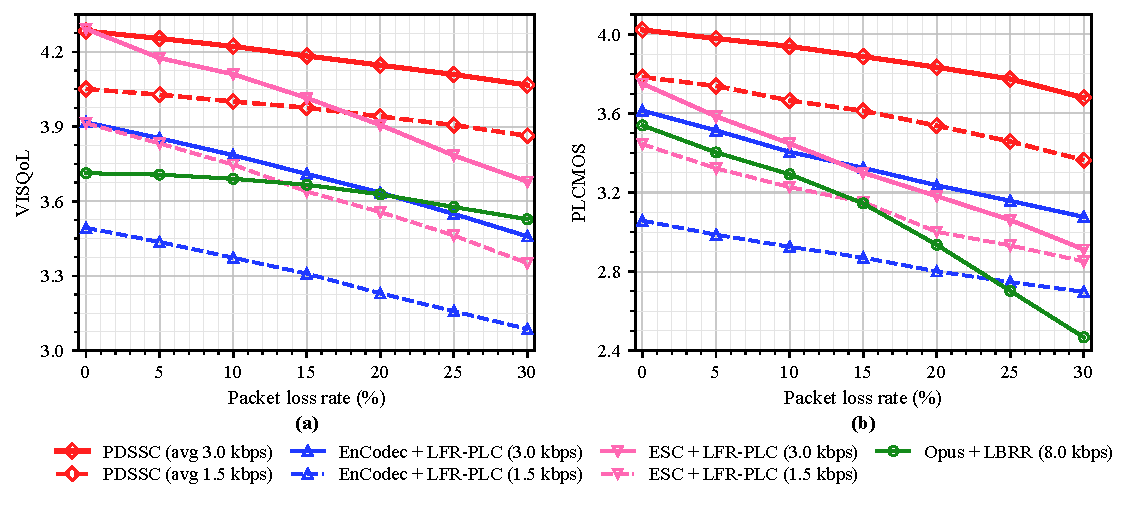
\includegraphics[width=1.05\linewidth]{paper_figs/fig6.pdf}}
\caption{Audio quality performance of PDSSC and competing methods under different packet loss rates: (a) ViSQOL, (b) PLCMOS.}
\label{fig:plr}
\end{figure}

The quantitative trends at average 3.0 and 1.5 kbps further support this robustness interpretation. At 3.0 kbps, PDSSC decreases only from 4.284 to 4.067 in ViSQOL and from 4.023 to 3.680 in PLCMOS across the full packet-loss interval, whereas EnCodec falls from 3.917 to 3.459 in ViSQOL and from 3.614 to 3.076 in PLCMOS, and ESC drops from 4.293 to 3.679 in ViSQOL and from 3.751 to 2.911 in PLCMOS. The same trend remains at 1.5 kbps, where the transmitted description is more incomplete from the outset and recovery is therefore more challenging. Even in this harsher regime, the PDSSC curves remain consistently above the corresponding EnCodec and ESC curves throughout the tested packet-loss range. This is consistent with the design logic of PDSSC: the more aggressive the bitrate reduction, the more valuable the targeted receiver-side recovery becomes. Another contributing factor is the hard-case-oriented training strategy, in which the low-rate operating points receive larger sampling emphasis and higher loss weight, further strengthening the model in the most fragile conditions.

We further isolate the role of the receiver-side completion model through the ablation results in Fig.~\ref{fig:ablation}. The effect is unambiguous: with flow completion, the curves consistently remain above those without flow over the whole packet-loss range, and the margin is substantial in both ViSQOL and PLCMOS. This confirms that the robustness gain in Fig.~\ref{fig:plr} does not arise simply from the layered codec itself, but critically depends on the receiver-side restoration model. In particular, the gain is especially pronounced in PLCMOS, showing that the flow model is highly effective in reconstructing the missing speaker-related and fine acoustic detail that governs perceptual continuity after packet erasure.

The stronger gains at lower bitrate are also consistent with the training objective of the flow model. The model is trained under different transmitted depths, but in all cases its target is the same complete latent $\mathbf{h}$. When fewer layers are transmitted, it must therefore compensate for a larger amount of missing high-layer information, and the value of speaker-prior-guided restoration becomes more prominent. This trend is clearly visible at the average 1.5 kbps operating point, where the gap between the versions with and without flow is larger than that at 3.0 kbps. For example, at 30\% packet loss, introducing the flow module improves ViSQOL from 3.739 to 3.865 and PLCMOS from 2.699 to 3.350 at 1.5 kbps, while the corresponding improvement at 3.0 kbps is from 3.969 to 4.070 in ViSQOL and from 3.263 to 3.700 in PLCMOS. Taken together, these results show that the proposed low-step flow completion model is what allows PDSSC to convert incomplete layered observations into stable high-quality recovery, especially in the most challenging low-rate conditions.

\begin{figure}[!t]
\makebox[\linewidth][c]{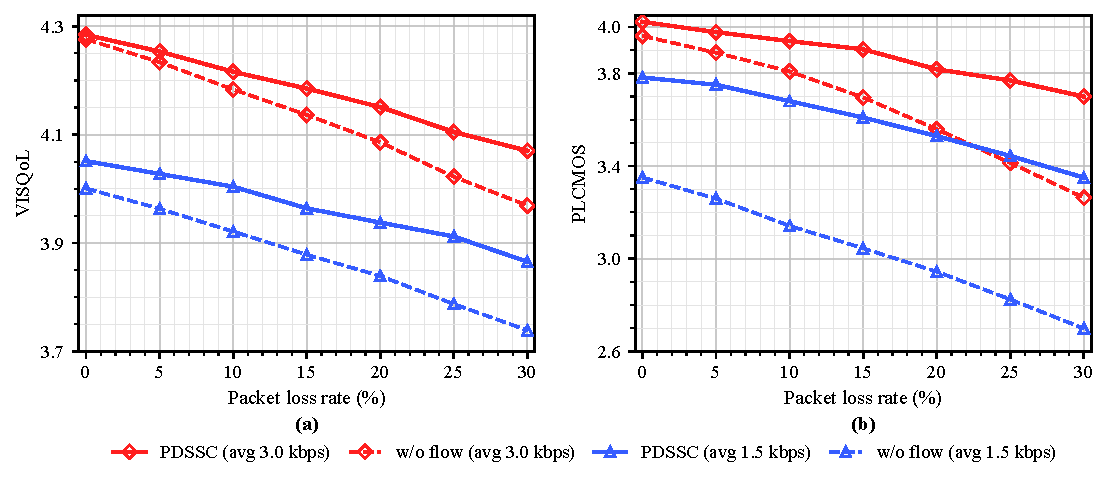
\includegraphics[width=1.05\linewidth]{paper_figs/fig8.pdf}}
\caption{Ablation results of the flow completion module under different packet loss rates: (a) ViSQOL, (b) PLCMOS.}
\label{fig:ablation}
\end{figure}

The same advantage is also visible from a qualitative time-frequency perspective. Fig.~\ref{fig:mel_compare} shows a representative mel-spectrogram comparison from the test set. The spectrum reconstructed by PDSSC remains visibly closer to the original signal, especially in the continuity of harmonic stripes and the preservation of formant trajectories. By contrast, the competing baselines show more pronounced over-smoothing, local blurring, or missing fine detail, consistent with the quantitative gains reported above.

\begin{figure}[!t]
\makebox[\linewidth][c]{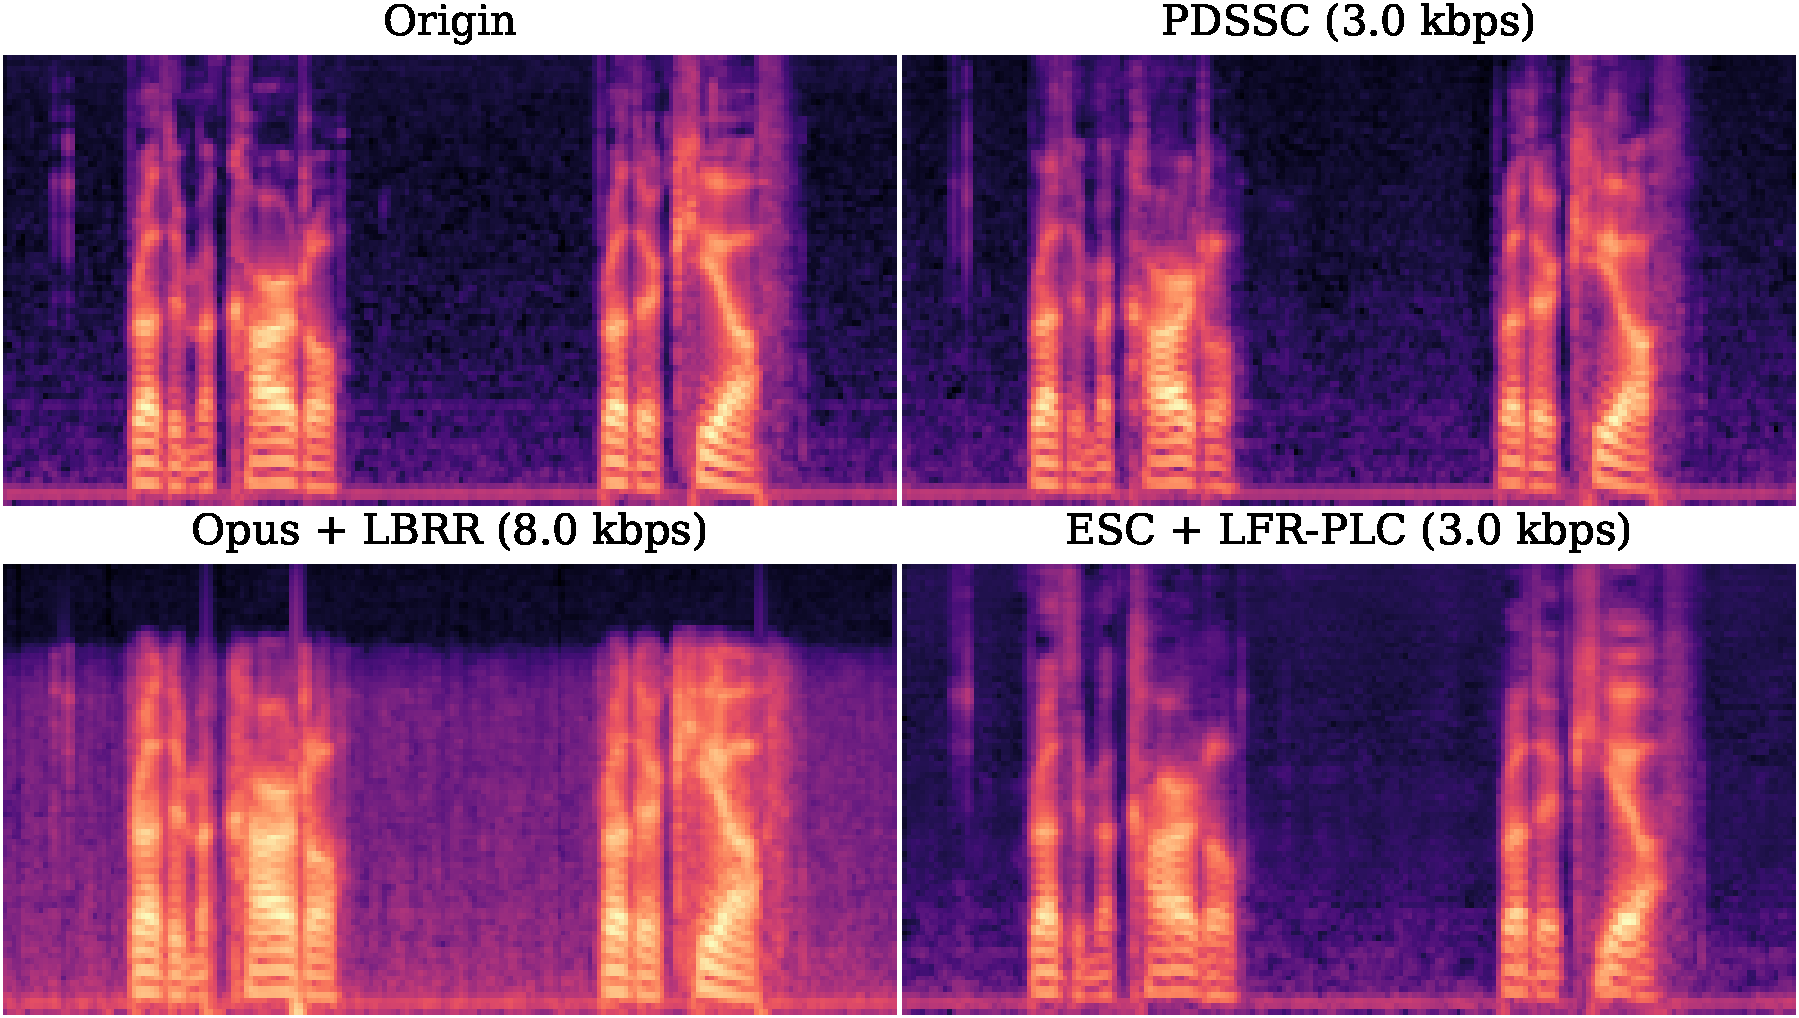
\includegraphics[width=0.98\linewidth]{paper_figs/fig7.pdf}}
\caption{Mel-spectrogram comparison of PDSSC and competing methods on a representative test case.}
\label{fig:mel_compare}
\end{figure}

Finally, we examine whether these gains remain compatible with practical deployment constraints. Tables~I and~II summarize the computational efficiency and real-time performance of PDSSC. Table~I shows that the dominant cost still lies in the semantic encoder and decoder, while the RVQ module contributes only moderate additional complexity and the adaptive controller adds almost negligible overhead. The flow completion model is clearly lighter than the full codec backbone, indicating that the robustness gain of PDSSC comes from a targeted completion mechanism rather than an excessively heavy receiver-side generator.

\begin{table}[!t]
\caption{Model complexity of the proposed PDSSC system.}
\label{tab:complexity}
\centering
\begin{tabular}{lcc}
\hline
Module & GFLOPs & Params (M) \\
\hline
Semantic Encoder & 58.694 & 103.676 \\
RVQ Codebooks & 4.198 & 8.389 \\
Adaptive Controller & 0.008 & 0.031 \\
Flow Completion Model & 11.726 & 58.470 \\
Semantic Decoder & 111.256 & 103.676 \\
Total & 185.882 & 274.242 \\
\hline
\end{tabular}
\end{table}

The latency comparison in Table~II further confirms the practical efficiency of the proposed design. At the same 3.0 kbps operating point, PDSSC achieves an average end-to-end delay of 0.151 s, which is markedly lower than ESC at 0.330 s, even though ESC is also a semantic low-bitrate baseline. It is also substantially faster than representative semantic communication systems such as SyncSC at 1.86 s and LargeSC at 0.46 s, further highlighting the real-time advantage of the proposed design. EnCodec remains faster at 0.103 s, but it does not provide the same level of low-bitrate quality and packet-loss robustness shown above. For reference, Opus + LBRR reaches 0.071 s at 8.0 kbps, indicating that conventional signal-reconstruction-based coding still benefits from a simpler pipeline when bitrate is substantially less constrained. Taken together, these results show that PDSSC attains a more favorable balance between restoration capability and deployment efficiency than existing semantic baselines, while remaining practical for real-time speech communication.

\begin{table}[!t]
\caption{End-to-end latency comparison of PDSSC and competing methods.}
\label{tab:latency}
\centering
\begin{tabular}{lccc}
\hline
Method & Sample rate (kHz) & Bitrate (bps) & Delay (s) \\
\hline
PDSSC & 16.0 & 3000 & 0.151 \\
EnCodec + LFR-PLC & 24.0 & 3000 & 0.103 \\
ESC + LFR-PLC & 16.0 & 3000 & 0.330 \\
SyncSC & 16.0 & 55.37 & 1.86 \\
LargeSC & 24.0 & 2060 & 0.46 \\
Opus + LBRR & 24.0 & 8000 & 0.071 \\
\hline
\end{tabular}
\end{table}

\section{Conclusion}
PDSSC addresses digital semantic speech communication over extremely low-bitrate and packet-loss-prone channels by combining a semantic-priority layered discrete representation, a speaker-prior-guided flow completion model, and lightweight bitrate control within one unified framework. This design enables progressive transmission, targeted receiver-side restoration, and flexible rate adaptation under constrained links. Experimental results show that PDSSC achieves a favorable quality-bitrate tradeoff, degrades more gracefully under packet loss than the compared baselines, and remains practical for real-time deployment. Future work will focus on lower-latency streaming completion, more flexible channel adaptation, and evaluation under more realistic wireless conditions.

\begin{thebibliography}{00}

\bibitem{3gpp_ntn} 3GPP, ``Non-terrestrial networks (NTN),'' accessed May 12, 2026. [Online]. Available: \url{https://www.3gpp.org/technologies/ntn-overview}

\bibitem{cheng2022sagin} N. Cheng, W. Quan, W. Shi, H. Wu, and X. Shen, ``Space-air-ground integrated network (SAGIN) for 6G: Requirements, architecture, and challenges,'' \emph{IEEE Communications Magazine}, vol. 60, no. 11, pp. 90--96, Nov. 2022.

\bibitem{ngmn_ntn} NGMN Alliance, ``Non-terrestrial networks position paper,'' 2023. [Online]. Available: \url{https://www.ngmn.org/publications/ntn-position-paper.html}

\bibitem{guler2018semantic} B. Guler, A. Yener, and A. Swami, ``The semantic communication game,'' \emph{IEEE Transactions on Cognitive Communications and Networking}, vol. 4, no. 4, pp. 787--802, Dec. 2018.

\bibitem{xie2021deepsc} H. Xie, Z. Qin, G. Y. Li, and B.-H. Juang, ``Deep learning enabled semantic communication systems,'' \emph{IEEE Transactions on Signal Processing}, vol. 69, pp. 2663--2675, 2021.

\bibitem{iso_aac} ISO/IEC, ``Information technology -- Coding of audio-visual objects -- Part 3: Audio,'' ISO/IEC 14496-3:2019, 2019.

\bibitem{valin2012opus} J.-M. Valin, K. Vos, and T. Terriberry, ``Definition of the Opus audio codec,'' IETF RFC 6716, Sept. 2012.

\bibitem{xiao2023dsst} Z. Xiao, S. Yao, J. Dai, S. Wang, K. Niu, and P. Zhang, ``Wireless deep speech semantic transmission,'' in \emph{Proc. IEEE International Conference on Acoustics, Speech and Signal Processing (ICASSP)}, 2023.

\bibitem{defossez2023encodec} A. D\'efossez, J. Copet, G. Synnaeve, and Y. Adi, ``High fidelity neural audio compression,'' \emph{Transactions on Machine Learning Research}, 2023.

\bibitem{chen2025rvqgan} X. Chen, J. Wang, J. Huang, M. Zeng, Z. Zheng, and Z. Fei, ``Low-bitrate high-quality digital semantic communication based on RVQGAN,'' \emph{IEEE Internet of Things Journal}, vol. 12, no. 10, pp. 13525--13537, 2025.

\bibitem{tian2025lsm} Y. Tian, Z. Qin, G. Lv, Y. Jin, K. Huang, and Z. Han, ``Large speech model enabled semantic communication,'' arXiv:2512.04711, 2025.

\bibitem{han2025esc} Z. Han, J. Dai, S. Yao, J. Wang, Y. Li, K. Niu, W. Xu, and P. Zhang, ``Error-resilient semantic communication for speech transmission over packet-loss networks,'' arXiv:2512.08203, 2025.

\bibitem{oord2017vqvae} A. van den Oord, O. Vinyals, and K. Kavukcuoglu, ``Neural discrete representation learning,'' in \emph{Proc. Advances in Neural Information Processing Systems (NeurIPS)}, 2017.

\bibitem{lipman2023flow} Y. Lipman, R. T. Q. Chen, H. Ben-Hamu, M. Nickel, and M. Le, ``Flow matching for generative modeling,'' in \emph{Proc. International Conference on Learning Representations (ICLR)}, 2023.

\bibitem{panayotov2015librispeech} V. Panayotov, G. Chen, D. Povey, and S. Khudanpur, ``LibriSpeech: An ASR corpus based on public domain audio books,'' in \emph{Proc. IEEE International Conference on Acoustics, Speech and Signal Processing (ICASSP)}, 2015, pp. 5206--5210.

\bibitem{hines2015visqol} A. Hines, J. Skoglund, A. C. Kokaram, and N. Harte, ``ViSQOL: An objective speech quality model,'' \emph{EURASIP Journal on Audio, Speech, and Music Processing}, vol. 2015, no. 1, article 13, 2015.

\bibitem{saeki2022utmos} T. Saeki, D. Xin, W. Nakata, T. Koriyama, S. Takamichi, and H. Saruwatari, ``UTMOS: UTokyo-SaruLab system for VoiceMOS Challenge 2022,'' in \emph{Proc. Interspeech}, 2022.

\bibitem{diener2023plcmos} L. Diener, M. Purin, S. Sootla, A. Saabas, R. Aichner, and R. Cutler, ``PLCMOS -- A data-driven non-intrusive metric for the evaluation of packet loss concealment algorithms,'' in \emph{Proc. Interspeech}, 2023, pp. 2533--2537.

\end{thebibliography}

\end{document}
